\begin{figure}[p]\centering
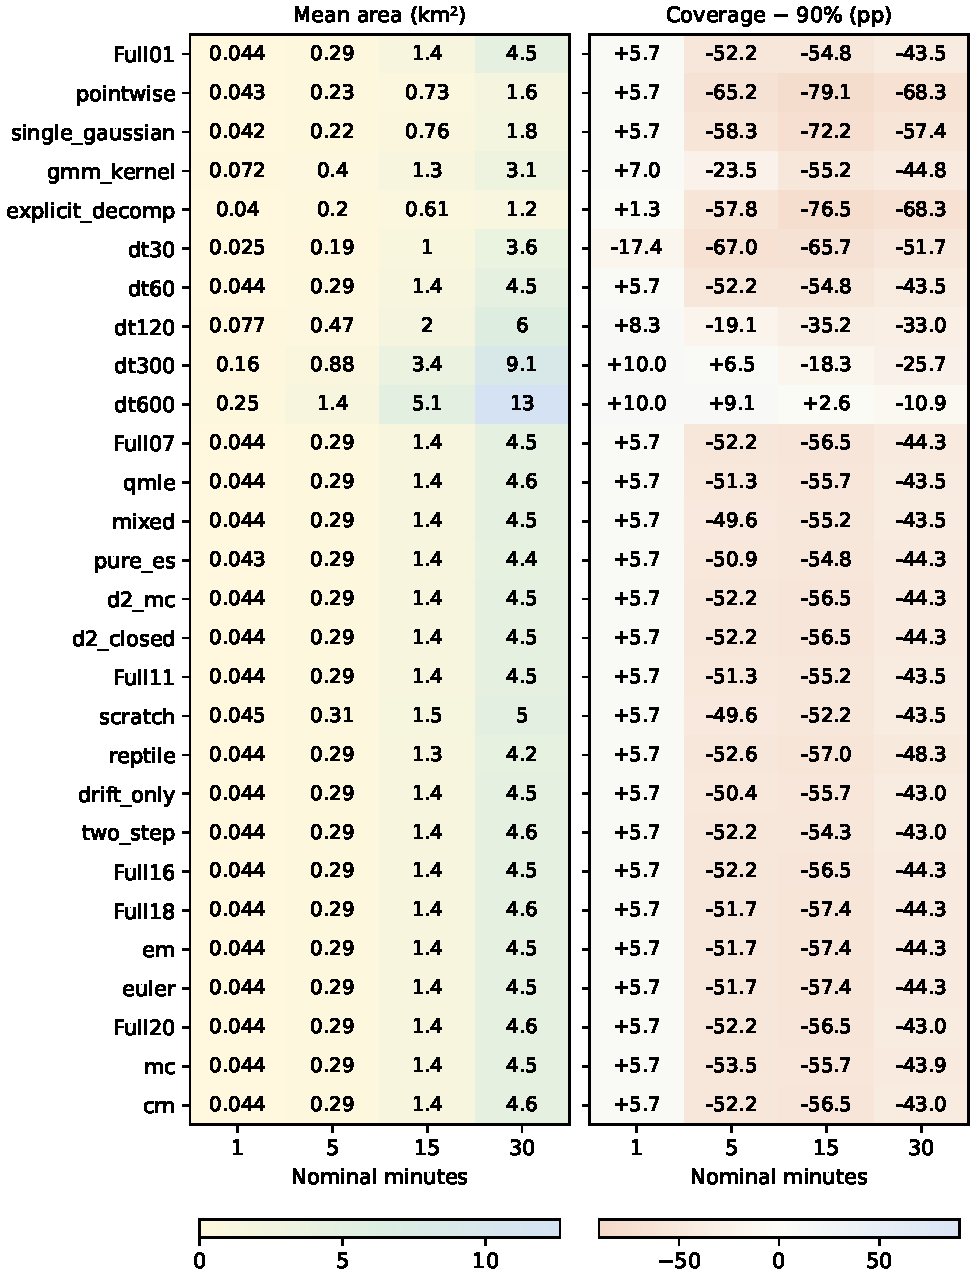
\includegraphics[height=.79\textheight,width=\linewidth,keepaspectratio]{../figures/reader-v2/method-region-overview.pdf}
\caption{28 configurations, four horizons, two metrics: 224 scalar cells.
Left: mean 90\% disk area (km$^2$), with a linear scale shared with the main
overview. Right: coverage minus 90\% (percentage points), with a symmetric
zero-centred scale. Neither area nor coverage is a standalone quality rank.
Each cell averages seeds within each of 46 blocks, then weights blocks
equally. Area averages individual disk areas, not the square of mean radius.
The same cohort and forecasts underlie the other overviews; repeated views
are not independent evidence. Full values are in Table~\ref{tab:all-method-regions}.}
\label{fig:all-method-regions}\end{figure}
